\documentclass{article}
\usepackage{listings}             % Include the listings-package
\usepackage[utf8x]{inputenc} % Allow utf-8 characters in the tex document
\usepackage{geometry}
\usepackage{float}
\usepackage[most]{tcolorbox} %apply colors on background
    
    \tcbset{	%background color configuration
    frame code={}
    center title,
    left=0pt,
    right=0pt,
    top=0pt,
    bottom=0pt,
    colback=gray!30,
    colframe=white,
    width=\dimexpr\textwidth\relax,
    enlarge left by=0mm,
    boxsep=5pt,
    arc=0pt,outer arc=0pt,
    }

\title{Exercício 7 - MO444 - Aprendizado de máquina e reconhecimento de padrões}
\date{}
\author{Renato Lopes Moura - 163050}
    
\geometry{verbose,tmargin=0.3in,bmargin=0.3in,lmargin=0.25in,rmargin=0.25in}

% Default fixed font does not support bold face
\DeclareFixedFont{\ttb}{T1}{txtt}{bx}{n}{9} % for bold
\DeclareFixedFont{\ttm}{T1}{txtt}{m}{n}{9}  % for normal

% Custom colors
\usepackage{color}
\definecolor{deepblue}{rgb}{0,0,0.5}
\definecolor{deepred}{rgb}{0.6,0,0}
\definecolor{deepgreen}{rgb}{0,0.5,0}

% Python style for highlighting
\newcommand\pythonstyle{\lstset{
language=Python,
basicstyle=\ttm,
otherkeywords={self},             % Add keywords here
keywordstyle=\ttb\color{deepblue},
emph={MyClass,__init__},          % Custom highlighting
emphstyle=\ttb\color{deepred},    % Custom highlighting style
stringstyle=\color{deepgreen},
frame=tb,                         % Any extra options here
showstringspaces=false            % 
}}


% Python environment
\lstnewenvironment{python}[1][]
{
\pythonstyle
\lstset{#1}
}
{}

% Python for external files
\newcommand\pythonexternal[2][]{{
\pythonstyle
\lstinputlisting[#1]{#2}}}

% Python for inline
\newcommand\pythoninline[1]{{\pythonstyle\lstinline!#1!}}

\begin{document}

\maketitle

\section{Código}
\subsection{Leitura de dados}
%\lstinputlisting[language=Python]{ex5.py}
\begin{tcolorbox}
\begin{python}
import numpy as np
import pandas as pd
import matplotlib.pyplot as plt 
import math

#Leitura dos dados dos arquivos csv utilizando o pandas
dados1 = pd.read_csv('serie1.csv')
dados2 = pd.read_csv('serie2.csv')
dados3 = pd.read_csv('serie3.csv')
dados4 = pd.read_csv('serie4.csv')
dados5 = pd.read_csv('serie5.csv')

#Conversao dos dataframes do pandas para arrays do numpy
array1 = dados1.values
array2 = dados2.values
array3 = dados3.values
array4 = dados4.values
array5 = dados5.values
\end{python}
\end{tcolorbox}

\newpage

\subsection{Funções de apoio e métodos de detecção}
\begin{tcolorbox}
\begin{python}
###############################################################################
#Funcao para calcular a media e desvio padrao de parte da serie
def meanAndStd(series, n):
	mean = np.mean(series[0:n-1], axis=0)
	std = np.std(series[0:n-1], axis=0)
	return mean, std

#Metodo 1: verifica se existem valores fora da margem:
# media +/- desvio padrao +/- tolerancia (= 3 desvios padrao)
def method1(mean, std, tol, array):
	for i in range(0,array.shape[0]):
		if array[i,1] > (mean+std+tol):
			print "anomalia encontrada em "+str(i)+" valor "+str(array[i,1])
			anomalia = i
			break
		elif array[i,1] < (mean-std-tol):
			print "anomalia encontrada em "+str(i)+" valor "+str(array[i,1])
			anomalia = i
			break
	return anomalia

#Metodo 2: tenta encontrar o tamanho da janela de repeticao da serie (chunk)
# e depois calcula a media de cada chunk procurando por chunks com anomalia
def method2(mean, tol_mean, array):
	chunk = 1

	#Tenta determinar o tamanho do chunk
	for i in np.arange(0,array.shape[0],10):
		if np.mean(array[0:chunk,1]) > (mean+tol_mean):
			chunk = chunk+10
		elif np.mean(array[0:chunk,1]) < (mean-tol_mean):
			chunk = chunk+10
		elif (np.mean(array[0:3*chunk,1]) < (mean+tol_mean)) and (np.mean(array[0:3*chunk,1]) > (mean-tol_mean)):
			#Verifica se o tamanho do chunk esta certo calculando a media de 3 chunks
			break
		else:
			chunk = chunk+10

	print "chunk size: "+str(chunk)

	n_chunks = int(math.floor(array.shape[0]/chunk))

	#Calcula a media chunk por chunk em busca de anomalias
	for i in range(0,n_chunks):
		ini = chunk*i
		end = chunk*(i+1)

		if np.mean(array[ini:end,1]) > (mean+tol_mean):			
			anomalia = int(math.floor((ini+end)/2))
			print "anomalia encontrada em torno de "+str(anomalia)+" media "+str(np.mean(array[ini:end,1]))
			break
		elif np.mean(array[ini:end,1]) < (mean-tol_mean):
			anomalia = int(math.floor((ini+end)/2))
			print "anomalia encontrada em torno de "+str(anomalia)+" media "+str(np.mean(array[ini:end,1]))
			break

	return anomalia
\end{python}
\end{tcolorbox}
\newpage
\begin{tcolorbox}
\begin{python}
#Metodo 3: calcula o log da serie e a media movel,
# e entao procura pontos onde a media movel foge do intervalo de tolerancia
def method3(array):
	serie_log = np.log10(array[:,1].astype(float)+1)
	moving_avg = pd.Series(serie_log).rolling(window=10).mean()
	mean_moving = np.mean(moving_avg, axis=0)
	std_moving = np.std(moving_avg, axis=0)
	tol_moving = 3*std_moving

	print "mean moving "+str(mean_moving)
	print "std moving "+str(std_moving)

	for i in range(0,moving_avg.shape[0]):
		if moving_avg[i] > (mean_moving+std_moving+tol_moving):
			print "anomalia encontrada em "+str(i)+" valor "+str(array[i,1])
			anomalia = i
			break
		elif moving_avg[i] < (mean_moving-std_moving-tol_moving):
			print "anomalia encontrada em "+str(i)+" valor "+str(array[i,1])
			anomalia = i
			break
	return anomalia

\end{python}
\end{tcolorbox}

\newpage

\subsection{Aplicação dos métodos nas séries}
\begin{tcolorbox}
\begin{python}
################################################################################
#Serie 1
#Calcula a media e desvio padrao da serie 1 considerando os 25% primeiros dados
mean1,std1 = meanAndStd(array1[:,1], array1.shape[0]/4)
tol1 = 3*std1

print "mean serie 1: "+str(mean1)
print "std serie 1: "+str(std1)

anomalia1 = method1(mean1, std1, tol1, array1)

print "\n"

################################################################################
#Serie 2
#Calcula a media e desvio padrao da serie 2 considerando os 25% primeiros dados
mean2,std2 = meanAndStd(array2[:,1], array2.shape[0]/4)
tol_mean2 = 0.05*mean2

print "mean serie 2: "+str(mean2)
print "std serie 2: "+str(std2)
print "mean + tol serie 2: "+str(mean2+tol_mean2)
print "mean - tol serie 2: "+str(mean2-tol_mean2)

anomalia2 = method2(mean2, tol_mean2, array2)

print "\n"

################################################################################
#Serie 3
#Calcula a media e desvio padrao da serie 3 considerando os 25% primeiros dados
mean3,std3 = meanAndStd(array3[:,1], array3.shape[0]/4)
tol_mean3 = 0.05*mean3

print "mean serie 3: "+str(mean3)
print "std serie 3: "+str(std3)
print "mean + tol serie 3: "+str(mean3+tol_mean3)
print "mean - tol serie 3: "+str(mean3-tol_mean3)

anomalia3 = method2(mean3, tol_mean3, array3)

print "\n"

################################################################################
#Serie 4
#Calcula a media e desvio padrao da serie 4 considerando os 25% primeiros dados
mean4,std4 = meanAndStd(array4[:,1], array4.shape[0]/4)

print "mean serie 4: "+str(mean4)
print "std serie 4: "+str(std4)

anomalia4 = method3(array4)

print "\n"
\end{python}
\end{tcolorbox}
\newpage
\begin{tcolorbox}
\begin{python}
################################################################################
#Serie 5
#Calcula a media e desvio padrao da serie 4 considerando os 25% primeiros dados
mean5,std5 = meanAndStd(array5[:,1], array5.shape[0]/4)
tol5 = 3*std5
tol_mean5 = 0.05*mean5

print "mean serie 5: "+str(mean5)
print "std serie 5: "+str(std5)

anomalia5_1 = method1(mean5, std5, tol5, array5)
anomalia5_2 = method2(mean5, tol_mean5, array5)
anomalia5_3 = method3(array5)

print "\n"
\end{python}
\end{tcolorbox}

\newpage

\subsection{Montagem dos gráficos}
\begin{tcolorbox}
\begin{python}
#################################################################################
#Graficos das series com as anomalias indicadas
fig, ((ax0, ax1), (ax2, ax3), (ax4, ax5)) = plt.subplots(nrows=3, ncols=2, figsize=(12,12))

#Grafico serie 1
x_ini_1 = array1.shape[0]/2
y_ini_1 = max(array1[:,1])+10
x_dist_1 = anomalia1 - x_ini_1 - 50
y_dist_1 = array1[anomalia1,1] - y_ini_1

ax0.plot(array1[:,1])
ax0.arrow(x_ini_1, y_ini_1, x_dist_1, y_dist_1, head_width=10, head_length=20, fc='r', ec='r')
ax0.set_title("Serie 1")

#Grafico serie 2
x_ini_2 = array2.shape[0]/2
y_ini_2 = max(array2[:,1])+10
x_dist_2 = anomalia2 - x_ini_2 - 50
y_dist_2 = array2[anomalia2,1] - y_ini_2

ax1.plot(array2[:,1])
ax1.arrow(x_ini_2, y_ini_2, x_dist_2, y_dist_2, head_width=10, head_length=20, fc='r', ec='r')
ax1.set_title("Serie 2")

#Grafico serie 3
x_ini_3 = array3.shape[0]/2
y_ini_3 = max(array3[:,1])+10
x_dist_3 = anomalia3 - x_ini_3 - 50
y_dist_3 = array3[anomalia3,1] - y_ini_3

ax2.plot(array3[:,1])
ax2.arrow(x_ini_3, y_ini_3, x_dist_3, y_dist_3, head_width=10, head_length=20, fc='r', ec='r')
ax2.set_title("Serie 3")

#Grafico serie 4
x_ini_4 = array4.shape[0]/2
y_ini_4 = max(array4[:,1])+10
x_dist_4 = anomalia4 - x_ini_4 - 20
y_dist_4 = array4[anomalia4,1] - y_ini_4

ax3.plot(array4[:,1])
ax3.arrow(x_ini_4, y_ini_4, x_dist_4, y_dist_4, head_width=2, head_length=3, fc='r', ec='r')
ax3.set_ylim([min(array4[:,1])-2,max(array4[:,1])+2])
ax3.set_title("Serie 4")
\end{python}
\end{tcolorbox}

\newpage

\begin{tcolorbox}
\begin{python}
#Grafico serie 5
x_ini_5_1 = array5.shape[0]/2
y_ini_5_1 = max(array5[:,1])+10
x_dist_5_1 = anomalia5_1 - x_ini_5_1 - 20
y_dist_5_1 = array5[anomalia5_1,1] - y_ini_5_1

x_ini_5_2 = array5.shape[0]/2
y_ini_5_2 = max(array5[:,1])+10
x_dist_5_2 = anomalia5_2 - x_ini_5_2 - 20
y_dist_5_2 = array5[anomalia5_2,1] - y_ini_5_2

x_ini_5_3 = array5.shape[0]/2
y_ini_5_3 = max(array5[:,1])+10
x_dist_5_3 = anomalia5_3 - x_ini_5_3 - 20
y_dist_5_3 = array5[anomalia5_3,1] - y_ini_5_3

ax4.plot(array5[:,1])
ax4.arrow(x_ini_5_1, y_ini_5_1, x_dist_5_1, y_dist_5_1, head_width=0.5, head_length=1, fc='r', ec='r')
ax4.arrow(x_ini_5_2, y_ini_5_2, x_dist_5_2, y_dist_5_2, head_width=0.5, head_length=1, fc='r', ec='r')
ax4.arrow(x_ini_5_3, y_ini_5_3, x_dist_5_3, y_dist_5_3, head_width=0.5, head_length=1, fc='r', ec='r')
ax4.set_ylim([min(array5[:,1])-1,max(array5[:,1])+1])
ax4.set_title("Serie 5")

fig.delaxes(ax5)

plt.tight_layout()
plt.show()
\end{python}
\end{tcolorbox}

\newpage

\section{Outputs}
\begin{tcolorbox}
mean serie 1: 41.3726350546 \\
std serie 1: 27.8368952363 \\
anomalia encontrada em 3001 valor 159.259712824 \\
\\

mean serie 2: 41.3359316559 \\
std serie 2: 27.8713761877 \\
mean + tol serie 2: 43.4027282386 \\
mean - tol serie 2: 39.2691350731 \\
chunk size: 281 \\
anomalia encontrada em torno de 2950 media 27.7896540829 \\
\\

mean serie 3: 41.1263863637 \\
std serie 3: 27.5554321675 \\
mean + tol serie 3: 43.1827056819 \\
mean - tol serie 3: 39.0700670455 \\
chunk size: 281 \\
anomalia encontrada em torno de 2950 media 20.4934251525 \\
\\

mean serie 4: 0.436941410129 \\
std serie 4: 2.92368096869 \\
mean moving 0.0275421269945 \\
std moving 0.0674673437938 \\
anomalia encontrada em 2006 valor 20.0 \\
\\

mean serie 5: 0.0731622602537 \\
std serie 5: 0.351624113632 \\
anomalia encontrada em 180 valor 2.6516335011 \\
chunk size: 981 \\
anomalia encontrada em torno de 1471 media 0.0454836282884 \\
mean moving 0.0274748000801 \\
std moving 0.0603021741093 \\
anomalia encontrada em 2914 valor 2.6075039486

\end{tcolorbox}

\newpage

\section{Gráficos}
\begin{figure}[H]
  \centering
    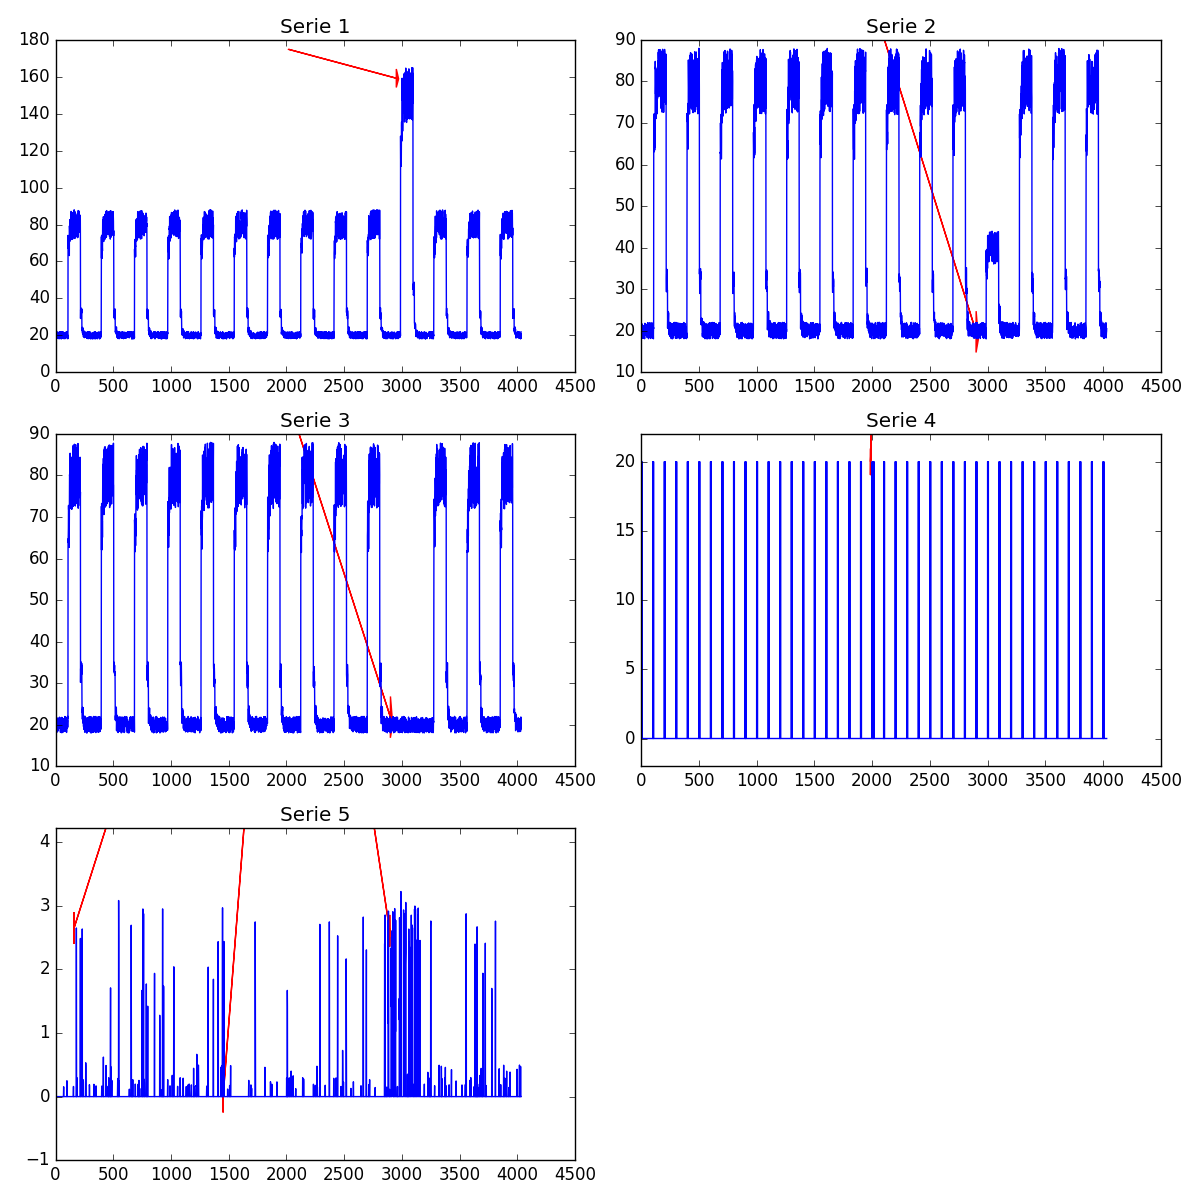
\includegraphics[scale=0.65]{graficos.png}
    \caption{Graficos das series com anomalias indicadas.}
\end{figure}

\end{document}